%% Select the dissertation mode on
%
% See the documentation for more information about the available class options 
% ('math', 'vertlayout', 'pdfa', ...)
% If you give option 'draft' or 'draft*', the draft mode is turned on
% NOTE if you want to generate abstracts for the publication platform, use
% the option 'abstracts'!
% The pdfa option is experimental, but give it a try -- your doc will be better archivable
%
\documentclass[dissertation,math,vertlayout,pdfa,colorlinks]{aaltoseries}

% Kludge to make sure we have utf8 input (check that this file is utf8!)
\makeatletter
\@ifpackageloaded{inputenc}{%
  \inputencoding{utf8}}{%
  \usepackage[utf8]{inputenc}}
\makeatother

% for live links. Takes the above option 'colorlinks' (use 'hidelinks' if you want them black for print).
\usepackage{hyperref} 

% Lipsum package generates quasi latin filler text
\usepackage{lipsum}
% Set the document languages used
\usepackage[english]{babel}
% more math symbols and environments if needed
\usepackage{amsmath,amssymb,amsthm} 
% after amsmath to restore bad page breaks in the middle of equations... only for those in the know
\interdisplaylinepenalty=2500 
% Adjust math line spacing
\renewcommand*{\arraystretch}{1.2} % for array/matrix environments
\setlength{\jot}{8pt} % for split environment

\usepackage{listings} % neat printing of source code
\usepackage[indentfirst=false,vskip=3mm]{quoting} % flexible quotes and quotations
% Enable the following to suppress page headers and numbers on 
% content-less left (even-numbered) pages. Fixes a bug in aaltoseries
\usepackage{emptypage}
\usepackage[nobiblatex]{xurl}


%Mathematical notations used 
\usepackage{amsmath}
\usepackage{amsfonts}
\usepackage{mathtools}
\usepackage{bm}

\newcommand{\bw}{\bm{w}}
\newcommand{\bX}{\bm{X}}
\newcommand{\by}{\bm{y}}
\newcommand{\bD}{\mathcal{D}}
\newcommand{\bF}{\mathcal{F}}
\DeclareMathOperator{\eye}{\textbf{I}}

\DeclarePairedDelimiterX{\infdivx}[2]{[}{]}{%
	#1\;\delimsize\|\;#2%
}
\DeclareMathOperator{\KLt}{KL}
\newcommand{\KL}{\KLt\infdivx}
\DeclareMathOperator{\betapdf}{Beta}
\DeclareMathOperator{\bernoullipdf}{Bernoulli}
\DeclareMathOperator{\normalpdf}{N}
\DeclareMathOperator{\gammapdf}{Gamma}
\DeclareMathOperator{\new}{new}
\DeclareMathOperator{\old}{old}
\DeclareMathOperator{\E}{\mathbb{E}}
\DeclareMathOperator{\var}{var}
\newcommand{\tp}{^{\top}}



\usepackage{graphicx}
%%
%% There's a HUGE number of LaTeX packages. Whatever it is you need, search for a package first before rolling your own!
%%

% This is the way you may input and separately develop your individual chapters. Write, e.g., 
%
%	%\input{Ch1}
%	%\input{Ch2}
%	\input{Ch3}
%	%\input{Ch4}
%	%\input{Ch5}
%
% ...when editing only the third chapter. Compilation with pdflatex ('pdflatex dissertation') will then only output
% a thin dissertation containing only the third chapter, but properly formatted.
%
% You may leave of the .tex extension here...
%
%    Some definitions useful in producing this sort of documentation:
\chardef\bslash=`\\ % p. 424, TeXbook
%    Normalized (nonbold, nonitalic) tt font, to avoid font
%    substitution warning messages if tt is used inside section
%    headings and other places where odd font combinations might
%    result.
\newcommand{\ntt}{\normalfont\ttfamily}
%    command name
\newcommand{\cn}[1]{{\protect\ntt\bslash#1}}
%    LaTeX package name
\newcommand{\pkg}[1]{{\protect\ntt#1}}
%    File name
\newcommand{\fn}[1]{{\protect\ntt#1}}
%    environment name
\newcommand{\env}[1]{{\protect\ntt#1}}
\hfuzz1pc % Don't bother to report overfull boxes if overage is < 1pc

%       Theorem environments

%% \theoremstyle{plain} %% This is the default
\newtheorem{thm}{Theorem}[section]
\newtheorem{cor}[thm]{Corollary}
\newtheorem{lem}[thm]{Lemma}
\newtheorem{prop}[thm]{Proposition}
\newtheorem{ax}{Axiom}

\theoremstyle{definition}
\newtheorem{defn}{Definition}[section]

\theoremstyle{remark}
\newtheorem{rem}{Remark}[section]
\newtheorem*{notation}{Notation}

%\numberwithin{equation}{section}

\newcommand{\thmref}[1]{Theorem~\ref{#1}}
\newcommand{\secref}[1]{\S\ref{#1}}
\newcommand{\lemref}[1]{Lemma~\ref{#1}}

\newcommand{\bysame}{\mbox{\rule{3em}{.4pt}}\,}

%       Math definitions

\newcommand{\A}{\mathcal{A}}
\newcommand{\BB}{\mathcal{B}}
\newcommand{\st}{\sigma}
\newcommand{\XcY}{{(X,Y)}}
\newcommand{\SX}{{S_X}}
\newcommand{\SY}{{S_Y}}
\newcommand{\SXY}{{S_{X,Y}}}
\newcommand{\SXgYy}{{S_{X|Y}(y)}}
\newcommand{\Cw}[1]{{\hat C_#1(X|Y)}}
\newcommand{\GG}{{G(X|Y)}}
\newcommand{\PY}{{P_{\mathcal{Y}}}}
\newcommand{\X}{\mathcal{X}}
\newcommand{\wt}{\widetilde}
\newcommand{\wh}{\widehat}

\DeclareMathOperator{\per}{per}
\DeclareMathOperator{\cov}{cov}
\DeclareMathOperator{\non}{non}
\DeclareMathOperator{\cf}{cf}
\DeclareMathOperator{\add}{add}
\DeclareMathOperator{\Cham}{Cham}
\DeclareMathOperator{\IM}{Im}
\DeclareMathOperator{\esssup}{ess\,sup}
\DeclareMathOperator{\meas}{meas}
\DeclareMathOperator{\seg}{seg}

%    \interval is used to provide better spacing after a [ that
%    is used as a closing delimiter.
\newcommand{\interval}[1]{\mathinner{#1}}

%    Notation for an expression evaluated at a particular condition. The
%    optional argument can be used to override automatic sizing of the
%    right vert bar, e.g. \eval[\biggr]{...}_{...}
\newcommand{\eval}[2][\right]{\relax
  \ifx#1\right\relax \left.\fi#2#1\rvert}

%    Enclose the argument in vert-bar delimiters:
\newcommand{\envert}[1]{\left\lvert#1\right\rvert}
\let\abs=\envert

%    Enclose the argument in double-vert-bar delimiters:
\newcommand{\enVert}[1]{\left\lVert#1\right\rVert}
\let\norm=\enVert



% The author of the dissertation
\author{Pedram Daee}
% The title of the thesis
\title{Interactive user modelling for human-in-the-loop machine learning} % This is the title of our line of work as a group.

%Comments from meeting with Sami on 15.07.2019:
% "user modelling" may not be the best term as people may perceive it as a statitstic UM. But "probabilistic user modelling" in a good context may be OK.
%  We want to have User + probabilistic in the title.
% Alternatives for user could be human-in-the-loop or user interaction or HCI or modellign of the user or interactive user modelling
% an alternative title could be to directly mention what I did: knowledge elicitation or multi source feedback. Or use these as subtitles?


%Keywords: Interactive intent modelling, User modelling, Interactive knowledge elicitation, Active elicitation of knowledge, Sequential probabilistic inference, high dimensional prediction.
%0. Probabilistic user modelling methods for improving human-in-the-loop machine learning
%1.	Probabilistic User Modelling in Interactive Machine Learning for Prediction
%2.	Machine learning methods for user modelling for improved prediction.
%3.	Interactive user/expert modelling for improved prediction 
%4.	Machine Learning Methods for Improved Prediction through Probabilistic User Modelling
%5.	Improved Prediction through Interactive Probabilistic User Modelling
%6.	Probabilistic user modelling methods for improving human-in-the-loop machine learning.

%Other comments: I do not like knowledge elicitation since it seems like a term that may become obsolete through time

\begin{document}

%% The abstract of the dissertation in English
% Use this command!
%\draftabstract{\lipsum[1-2]}%
%\draftabstract[english]{\hspace{-2pt} My abstract in English}
% Let's add another one in Finnish
%\draftabstract[finnish]{\hspace{-2pt} En puhu suomea1

%}%


% And yet another one in Swedish
%\draftabstract[swedish]{\lipsum[7-9]}
%%---------------------

%% The abstract of the dissertation in English
% Use this command!
%\begin{abstract}\lipsum[1-3]\end{abstract}%
% Let's add another one in Finnish

\begin{abstract}[english]
	Ongoing title: \\
	\textbf{Probabilistic user modelling methods for improving human-in-the-loop machine learning}
	
	\textbf{Interactive user modelling for human-in-the-loop machine learning} % NOTE: Interactive and in-the-loop are a bit redundant
	
	
	
	
	
%early comments from Sami: Drop half of the abstract and put it in the intro. Go into the gist and why it is different and what is done immediately. Sami thinks that the gist is “joint model of human and data through active learning, experimental design on a budget”. Add one sentence why it is a hard problem, then add another sentence that “and that is why we …..” to connect to your contribution. Sami thinks that intent modelling in IR is not prediction, but we model and solved it as a prediction problem. Maybe have “relevance of variables” as a keyword since this may be what I am doing. Regarding the title, keep the spirit but focus more. E.g., “human intent modelling for eliciting importance of variables” (knowledge elicitation?). Try to list 5 example titles and then have a meeting with Sami.
\end{abstract}

%1. What is the bigger picture?
%2. Dissertation purpose
%3. Research method
%4. Key results
%5. Practical Implications

%Typically 3 paragraphs: 1. the introduction of the challenge problem, 2. thesis, 3. contribution

 
\begin{abstract}%[finnish]
En puhu suomea.
\end{abstract}


% And yet another one in Swedish
%\begin{abstract}[swedish]\lipsum[7-9]\end{abstract}


%% Preface
% If you write this somewhere else than in Helsinki, use the optional location.
\begin{preface}[Espoo]
To fill.
%Maybe consider whom you should acknowledge. 
% at the very least, all the co-authors, group members who have worked in this or have acknowledge you in their theses, and the funding agencies (reknow, MindSee, WAI?)

\end{preface}

%% Table of contents of the dissertation
\clearpage
\tableofcontents

% To be defined before generating list of publications. Leave off if no acknowledgement
%\languagecheck{the Institute of Language Checks}

%% This is for article dissertations. Remove if you write a monograph dissertation.
% The actual publications are entered manually one by one as shown further down:
% use \addpublication, \addcontribution, \adderrata, and addpublicationpdf.
% The last adds the actual article, the other three enter related information
% that will be collected in lists -- like this one.
\listofpublications

%% Add lists of figures and tables as you usually do (\listoffigures, \listoftables)

%%%%%%%%%%%%%%%%%%%%%%% TODO: do I want to have the followings? Fig, table, Abb, sym? others did not have it.
%\listoffigures
%\listoftables

%\abbreviations
%\begin{description}
%\item[PDF] Probability Density Function
%\end{description}

%\symbols
%\begin{description}
%\item[$p(\theta \mid y)$] Conditional distribution
%\end{description}


%% The main matter, one can obviously use \input or \include
\chapter{Introduction}
%Comments from meeting with Sami on 15.07.2019:
% I need to tie to non-ML related works somewhere in the paper. This can include HCI related works or knowledge elicitation or multi agent? I need to either list them here and give a short descriotion or put them inside the next two chapters. In any case, I need to refer back to these in the Discussion section and mention how we improved the fields (and how we benefited from these).
% I need to also explain why probabilistic modelling is good 




%We can keep this empty and start from next. Alternatively we can write some stuff here and have only one section as "Contributions and organization of the thesis". See which one works better for you


Whether it is an everyday user searching for an application in her mobile phone or a doctor working with a cancer diagnostic system, humans and machines are increasingly interacting with each other \cite{amershi2014power} [more strong refs]. The goal of the thesis is to improve this interaction by incorporating a probabilistic model of the human user in the system they are interacting with. In particular, the thesis considers the family of problems where the human and machine interact to solve a prediction problem. Such problems can include personalized search activity or medical prediction about the response of a cancer drug. An important common factor in both these scenarios is that the number of labeled data (training data) that the machine can use to make predictions, is usually very few compared to the dimension of search space. This results in ill-posed statistical learning since there are limits in how low in sample size statistical methods can go \cite{Donoho2009observed}. 



%Copy-pasted text. I think we need to define user modelling here with some links to related works. 
\textcolor{red}{User modelling in human--computer interaction aims at improving the usability and usefulness of collaborative human--computer systems and providing personalised user experiences \cite{user_modelling_2001}. Machine learning based interactive systems extend user modelling to encompass statistical models interpreting user's actions.}


%\paragraph{Objective.}
%The objective of the thesis is to tackle the limited data problem by directly integrating a model of the human user into the modelling loop. The user can then provide more information about the problem (for example by giving feedback in response to the machine's query) that can help to improve the prediction performance. For example, in precision medicine obtaining additional data can be extremely costly or even impossible but the human knowledge, e.g., practitioners feedback, can be available and used to improve the prediction. My thesis proposes new probabilistic machine learning models to learn the human intent in interaction, new user models to learn about the knowledge of the human and accounting for common human biases, and new prediction models to employ and extract human knowledge to improve a task.


%\paragraph{Methodology.}
%USED FOR CHAPTER 2: I design probabilistic machine learning models to tie the data model (prediction model from the training data) to the user model (the model of the human) in a unified way. After doing so, we use Bayesian inference to find the posterior, i.e, distribution of the unknown parameters related to data and user, giving the training data and user interaction. The posterior inference, in most cases, does not have an analytical solution. We use different approximation methods, such as expectation propagation and variational inference, to handle the computation. 

%A core characteristic of the formulation is that the model adapts to the feedback obtained from the user and it sequentially integrates every piece of information before deciding on the next query for the user. This is important as humans can only answer limited number of queries (out of several thousands). The query selection is naturally formulated as experimental design problem, aiming at maximizing the most information gained, or multi-armed bandit problem, aiming at finding the most important piece of information, depending on the targeted task. For evaluation and testing, we conduct carefully designed user studies with real human.  



\section{Motivation}

%Thinking back, I think my main motivation should be on how to tackled limited interaction problem. In iui2016 we did it by adding new likelihoods, in JASIS by implicit interaction, in ML and IUI 18 by assuming strong priors.

%A) Small number of data ->add users

%B) user is the source of data

%Limited interaction: 1) need to be smart about what question to ask from the user 2) Should be able to consider all potential sources of feedback on different components of the interaction framework.


 
\section{Research questions and contributions}


This thesis investigates methods to tackle the limited user interaction challenge in interactive machine learning for prediction. The thesis focuses on scenarios where there is few labeled data available compared to the dimension of the problem, or when a human user is provider of the labeled data. The core idea of the thesis is to jointly model the human user with the data as part of a unified probabilistic model and use the model to improve the interaction.\\

\noindent \textbf{RQ1 --} \textit{Can we exploit new sources of interaction as additional learning signals from human user to improve interactive intent modelling?}

Publications I and V contribute to this research question by proposing models to incorporate new types of user feedback to amend the limited feedback in exploratory information seeking tasks. The tasks considered are document search scenarios where a user needs to sequentially provide relevance feedback to suggested keywords in order to find the targeted document. This is modelled as a multi-armed bandit problem with the goal of finding the most relevant document with minimum interaction. In particular, Publication I couples user relevance feedback on both documents and keywords by assuming a shared underlying latent model connected through a probabilistic model of the relationship between keywords and documents. Thompson sampling on the posterior of the latent intent was then used to recommend new documents and keywords in each iteration. Publication V investigates the use of implicit relevance feedback from neurophysiology signals for effortless information seeking. The work contributes by demonstrating how to integrate this inherently noisy and implicit feedback source with scarce explicit interaction. A model for controlling the accuracy of the feedback given its nature (implicit or explicit) was introduced. Similar to Publication I, Thompson sampling was used to control the exploration and exploitation balance of the recommendations. Both publications were evaluated by user studies in realistic information seeking tasks. 


\noindent \textbf{RQ2 --} \textit{Can expert knowledge about high dimensional data models be elicited to improve the prediction performance?}

Publications II and III contribute to this research question. Publication II proposes a framework for user knowledge elicitation as a probabilistic inference process, where the user knowledge is sequentially queried to improve predictions. In particular, sparse linear regression is considered as the data model with access to only few high-dimensional training data. It is assumed that there are experts who have knowledge about the relevance of the covariates, or of values of the regression coefficients and can provide this information to the data model if queried. The work contributes by an algorithm and computational approximation for fast and efficient interaction, which sequentially identifies the most informative queries to ask from the user. Publication III, builds on Publication II by adding user knowledge about direction of relevance of covariates and applying the method in important applications of precision medicine with the goal of predicting the effects of different treatments using high-dimensional genomic measurements. Both publications were evaluated by extensive simulations and user studies. 
Source codes for methods presented in Publications II and III, and user study data from Publication II are available at \\ \texttt{https://github.com/HIIT/knowledge-elicitation-for-linear-regression} and \\ \texttt{https://github.com/AaltoPML/knowledge-elicitation-for-precision-medicine}.




\noindent \textbf{RQ3 --} \textit{Is it enough to incorporate human knowledge directly in the data model as explained in RQ2, or could it be beneficial to account for rational knowledge updates that humans may undergo during the interaction?}

Publication IV contributes to this research question by modelling the knowledge provider, here the human user, as a rational agent that updates its knowledge about the underlying prediction task during the interaction. In particular, certain aspects of training data may be revealed to the user during knowledge elicitation. \textcolor{red}{The design of the system is then critical, since the elicited user knowledge cannot be assumed to be independent from the data model knowledge coming from the training data. If not accounted properly, knowledge elicitation can lead to double use of data and overfitting, if the user reinforces noisy patterns in the data. We propose a user modelling methodology, by assuming simple rational behaviour, to correct the problem and evaluate the method in a user study.} 
Source code and user study data are available at \texttt{https://github.com/HIIT/human-overfitting-in-IML}.

\section{Organization of the thesis}

The organization of the thesis is as follows. Chapter 2 provides an overview of probabilistic modelling and introduces our approach of modelling the user and \textcolor{red}{data} as a joint probabilistic model. Chapter three investigates the purpose of interactions and reviews different utility functions designed to minimize the effort of the user. The fourth chapter summarizes Publications I-IV. Chapter five concludes the thesis and provides discussions for future works.


%Comments from meeting with Sami on 15.07.2019:
% "data" usage is a bit awkward here as we are also modelling user interaction as new data. Maybe try to fine a better term?

\chapter{Probabilistic modelling of data and user} \label{prob_model_data_user}
% Sami's comments 15.07.2019: I need to also explain why probabilistic modelling is good and our approach for modelling the world. 

%I need to tie the chapters to RQs like what Antti did if I want to go with RQ type of thesis. "This chapter gives an overview of the line of research related to RQ1"

%TODO: lines should not start with a mathematical equation/formula/terms.
%TODO: use sequential ifnerence!

This chapter provides a brief introduction to probabilistic modelling as the main statistical framework that is used through the thesis. After some preliminaries,  Section \ref{prob_model_data} briefly reviews the type of linear models that are used in Publication I-IV for prediction. %  investigates linear models that are commonly used  for prediction.
Section \ref{prob_model_user} introduces different types of user interaction with the linear model and explains how user knowledge about the model can be incorporated as observational feedback. The computational solutions for Bayesian inference are reviewed in \ref{posteriro_inf}. Finally, the key components for modelling observational data and user feedback as a joint probabilistic model is introduced in Section \ref{key_comp}.

\section{Preliminaries}
The core idea of probabilistic modelling is to describe all the unobserved parameters and observed data as random variables from probability distributions. The unobserved parameters include the unknown quantity of interest or other parameters that affect the data or the quantity of interest. Bayesian inference provides a powerful framework to fit the described probabilistic model to observational data \cite{Gelman2013}. A core feature of Bayesian inference is that it provides probability distributions as the solution, compared to deterministic methods which provide a single outcome. This uncertainty quantification is of particularly high interest in cases where few observational data are available or when the data acquisition scheme is controlled by the model. Both of these constrains are prominently present in the tasks investigated by this thesis.

We follow the notation of \cite{Gelman2013} and use $p(.)$ to denote a probability distribution and $p(.\mid.)$ a conditional distribution. Consider the case where there are a set of observations $\bD= \{y_1,\ldots,y_n\}$ generated from a probabilistic model with an unobserved parameter of interest $\theta$. The observational model for an observation $y$ describes the conditional density of $y$ given the parameter $\theta$ and is denoted as $y \sim p(y \mid \theta)$. It is usually assumed that the observations are conditionally independent given $\theta$, enabling us to write the model for all observations as $p(\bD \mid \theta) =  \prod_{i=1}^{n} p(y_i \mid \theta)$. The observational model is called likelihood function if perceived as a function of $\theta$ with fixed observation $y$. One of the core questions in statistical inference is to estimate the parameter of interest $\theta$ based on observations $\bD$. % and the likelihood assumption. 
Bayesian inference answers this question by computing the conditional distribution of $\theta$ given $\bD$ following the Bayes rule


\begin{equation}\label{Eq:Bayes}
p(\theta \mid \bD) = \frac{p(\bD \mid \theta)p(\theta)}{p(\bD)}.
\end{equation}  

Where $p(\theta)$ represents the prior belief about $\theta$ and $p(\bD)$ is called the marginal likelihood and acts as a normalization factor as it does not depend on $\theta$. The marginal likelihood can be computed using the marginalization rule, i.e., $p(\bD)= \int_{\theta} p(\bD, \theta)d\theta= \int_{\theta} p(\bD \mid \theta)p(\theta) d\theta$ \footnote{The integral turns to summation for discrete $\theta$.}. $p(\theta \mid \bD)$ is called the posterior and it expresses the uncertainty surrounding the true value of $\theta$, after updating the prior assumptions about $\theta$ (i.e., the prior distribution) with the knowledge coming from the observations through the likelihood.  

In many cases, we may be more interested to make a prediction about an unknown observable data point $\hat{y}$ rather than the parameter $\theta$. Bayesian inference allows us to compute the conditional distribution of this unknown observable data given the observed data points by averaging over the posterior: 

\begin{equation}
p(\hat{y} \mid\bD ) = \int_{\theta} p(\hat{y}  \mid \theta)p(\theta \mid \bD)d\theta. 
\end{equation}

$p(\hat{y} \mid \bD)$ is known as the posterior predictive distribution and represents the uncertainty about a potential new observation. An example usage of this distribution could be when we want to predict the value of a test data. Since test data is unobserved, we can use posterior predictive distribution as our best guess. However, in many applications, only a value (and not a distribution) is required as the prediction. This can be handled by using some statistics of the distribution (for example mean or median) as the prediction. Still, the quantified uncertainty in the distribution can be useful as it provides knowledge about how certain we are about our estimate. Particularly, this uncertainty can help us to design more efficient interaction with a user, as will be discussed in Section \ref{interaction}.

	


\section{Modelling data for prediction} \label{prob_model_data}
%Alternative title: Prediction of high-diensional data?

Prediction is one of the core problems in statistical analysis and supervised machine learning. Given a set of $n$ input and output pairs, called training data, denoted by $\bD= \{(\bm{x}_i,y_i)\}_{i=1}^{n}$, the goal is to find a mapping from inputs to outputs. Here, $\bm{x}_i = [x_i^1,\ldots,x_i^d]\tp \in \mathbb{R}^d$ is a d-dimensional column vector representing the values of $i^{th}$ data point\footnote{We use subscripts to index an specific item (e.g, one particular observation out of several) and superscripts to refer to dimensions of the variable.}. The dimensions are commonly called feature, covariates, or attribute. $y_i$ is the corresponding response (or target) variable which can be anything depending on the underlying problem. In this thesis, we consider the regression tasks, meaning that we model response variables by real values, i.e., $y_i \in \mathbb{R}$. The problem is called classification in supervised learning if the response variable is restricted to categorical values (called classes). 

\subsection{Bayesian linear regression}

A well-studied and widely practical type of regression, known as linear regression, assumes that the relationship between all inputs and their corresponding response variables is linear. This relationship can be described as 

\begin{equation*}
y_i= \sum_{j=1}^{d}x_{i}^{j} w^{j}+\epsilon_i=\bm{x}_i\tp\bw+\epsilon_i, \qquad i=1,\ldots,n, 
\end{equation*}

\noindent where $\bw \in \mathbb{R}^d$ is the regression coefficients or the model's weights and $\epsilon_i$ is the residual error between linear prediction $\bm{x}_i\tp\bw$ and the response value $y_i$. Given the labeled data $\bD$, a commonly used error function is the sum of squared of residual errors $\sum_{i=1}^n(\bm{x}_i\tp\bw- y_i)^2$. By stacking the inputs in $\bX = [x_1,\ldots,x_n]\tp \in \mathbb{R}^{n\times d}$ and outputs in $\by = [y_1,\ldots,y_n]\tp \in \mathbb{R}^n$ the error can be expressed in vector format as $(\bX\bw- \by)\tp(\bX\bw- \by)$. The frequentist solution directly finds the point estimate for $\bw$ that minimizes this error (also known as least squares solution). It is straightforward to show that $\hat{\bw} = (\bX \tp \bX)^{-1}\bX\tp \by$  would be the point estimate solution given that $(\bX \tp \bX)^{-1}$ is invertible.  

However, as mentioned, we are interested in directly quantifying the uncertainty of the solution. The probabilistic way to model this problem is to explicitly describe the model assumptions (likelihood and priors) as probability distributions. In linear regression, the residual errors $\epsilon_i$ and the weights $\bw$ are modelled as random variables and the inputs $\bm{x}_i$ as vector of values that are given. A customary assumption is to model the residual errors as independent zero-mean Gaussian random variables $\epsilon_i \sim \normalpdf(0,\sigma^2)$, where $\sigma^2$ is variance of the Gaussian distribution which indicates the model tolerance about residual errors. It is common to also model $\sigma^2$ as another random variable with its own distribution assumption, however, we consider it to be a fixed hyperparameter for simplicity. The quantity of interest in the linear model is the regression coefficients. To complete the Bayesian inference loop, we need to consider a prior distribution on $\bw$. There are many ways to do this depending on the underlying task. One simple prior could be to assume that coefficients are independent and each come from a zero-mean Gaussian distribution, encouraging the weights to be close to zero. This simple Bayesian linear regression can be described by

\begin{align}\label{Eq:simple_Bayesian_regression} 
\by \sim \normalpdf(\bX\bw,\sigma^2 \eye),\\
\bw \sim \normalpdf(\textbf{0},\tau^2 \eye), \nonumber
\end{align}

\noindent where $\tau^2$ is the variance of the weights and $\eye$ is the identity matrix. For simplicity we assume that $\tau^2$ is also a fixed hyperparameter. Therefore, The only unobserved parameters of this model is $\bw$. The Bayesian rule allows us to derive the posterior for $\bw$ as\footnote{Note that we use $\bw \sim \normalpdf(0,\tau^2 \eye)$ to denote the random variable $\bw$ and $\normalpdf(\bw\mid 0,\tau^2 \eye)$ to refer to the density function.}

\begin{equation}\label{Eq:Bayes_rule_simple_reg}
p(\bw \mid \bD) = \frac{p(\bD \mid \bw)p(\bw)}{p(\bD)} = \frac{\normalpdf(\by \mid \bX \bw,\sigma^2 \eye) \normalpdf(\bw \mid 0,\tau^2 \eye))}{p(\bD)}.
\end{equation}  
%p(\bw \mid \bX , \by) = \frac{\normalpdf(\by \mid \bX \bw,\sigma^2 \eye) \normalpdf(\bw \mid 0,\tau^2 \eye))}{p(\bX , \by)}.

Generally, the posterior in many problems cannot be analytically derived (we will discuss this issue more in Section \ref{posteriro_inf}). For this simple model, however, an analytical solution is available. We will go through the steps as a exercise with posterior inference. Before starting, it would be useful to note that a multivariate Gaussian distribution can be expressed as  

\begin{align}\label{Eq:multi_Gauss}
\normalpdf(\bw \mid \bm{\mu},\bm{\Sigma}) &\propto \exp \left ((\bw - \bm{\mu})\tp\bm{\Sigma}^{-1}(\bw - \bm{\mu}) \right) \nonumber\\
&\propto \exp \left ( \bw\tp\bm{\Sigma}^{-1}\bw -  2\bw\tp\bm{\Sigma}^{-1}\bm{\mu} \right),
\end{align}

\noindent after dropping all the terms that are constant with respect to $\bw$. 

To derive the posterior, we follow Equation \ref{Eq:Bayes_rule_simple_reg} 

\begin{align} \label{Eq:lin_rel_simple_derivation}
p(\bw \mid \bD) &\propto \exp \left(\frac{1}{2\sigma^2} (\by - \bX \bw)\tp(\by - \bX \bw)\right) \exp(\frac{1}{2\tau^2}\bw\tp\bw) \nonumber\\ 
&\propto \exp \left (\sigma^{-2}(\by\tp\by - 2\bw\tp\bX\tp\by + \bw\tp\bX\tp\bX\bw)+ \tau^{-2}\bw\tp\bw \right) \nonumber\\
&\propto \exp \left ( -2\sigma^{-2}\bw\tp\bX\tp\by + \bw\tp( \sigma^{-2}\bX\tp\bX + \tau^{-2} \eye )\bw \right) %\\
%&= \exp \left ( -2\sigma^{-2}\bw\tp\bX\tp\by + \bw\tp\Sigma^{-1}\bw \right)
\end{align}    
 
\noindent where we dropped $p(\bD)$ and all the other terms which where constant with respect to $\bw$. Equation \ref{Eq:lin_rel_simple_derivation} has the same form to Equation \ref{Eq:multi_Gauss} (with respect to $\bw$) and therefore is proportional to a multivariate Gaussian distribution. This relation shows that the posterior should be multivariate Gaussian, as both equations should integrate to one, and thus its parameters can be found by matching the terms of the two equations as $\bm{\Sigma}^{-1} = ( \sigma^{-2}\bX\tp\bX + \tau^{-2} \eye ) $ and $\bm{\Sigma}^{-1}\bm{\mu} = \sigma^{-2}\bX\tp\by$. Finally, the posterior of our simple linear regression can be described as 

\begin{align}\label{Eq:lin_rel_simple_posterior}
	p(\bw \mid \bD) &= \normalpdf(\bw \mid \bm{\mu},\bm{\Sigma}), \text{where}\\
	\bm{\Sigma}^{-1} &= (\sigma^{-2}\bX\tp\bX + \tau^{-2} \eye ), \nonumber\\
	\bm{\mu} &= \bm{\Sigma}\sigma^{-2}\bX\tp\by. \nonumber
\end{align}

This simple Bayesian regression is used as the underlying data model in Publication I. It would be interesting to compare a point estimate of the posterior distribution with the frequentist solution $\hat{\bw} = (\bX \tp \bX)^{-1}\bX\tp \by$. Maximum a posteriori (MAP) is a point estimate which represents the value in the posterior that has the highest density. In our case, this would be equal to the posterior mean, which after some rearrangement, can be described as $\hat{\bw}_{MAP} = (\bX\tp\bX + \frac{\sigma^{2}}{\tau^{2}} \eye )^{-1}(\bX\tp\by)$. Comparing the mean of the posterior with the frequentist solution indicates that the two estimates are very similar with the only difference that the MAP estimate has the additive term $\frac{\sigma^{2}}{\tau^{2}} \eye$ in the covariance matrix. This added term is the direct outcome of our assumptions in the likelihood and prior of the model which were not present in our simple frequentist model. This term can also be interpreted as a regularization parameter that controls the variance of weights. The designer of the model may want to consider different types of regularization or constrains in the model, which in probabilistic modelling is usually done by incorporating them in the prior distribution. Such problems may not have an analytical posterior available. We will consider two such models in the following subsections.




\subsubsection{Sparsity-inducing priors}

In many prediction problems, in particular those that require human intervention in a form, the number of available training data is smaller than dimensions of the problem. If not regularized properly, a model trained in this setting may overfit to the training data (achieving very low training error) while not being able to generalize properly to unobserved data (high test data error). One way to tackle this challenge, is to directly regularize the model parameters so that they would not overfit. This regularization can be done by adding penalty terms, for example $l_1$ norms of the weights, to the error function in the non-Bayesian models with the general idea of pushing weights that are not useful toward zero (see for example Lasso \cite{lasso2011}). In probabilistic modelling, we can achieve the same goal by selecting sparsity-inducing priors. 

There are different priors that encourage sparsity but they can be categorized to two general groups of mixture priors, such as spike-and-slab prior \cite{spike_slab1993}, and the continuous shrinkage priors, such as horseshoe \cite{horseshoe_2017} and Laplace prior \cite{seeger2008bayesian}. The core idea of these priors is that their densities for coefficients peak at zero but at the same time have good amount of probability mass in non-zero values. In this thesis we consider the spike-and-slab prior as it introduces a binary latent variable that explicitly indicates whether a coefficient should be zero or non-zero  (relevant and not-relevant groups). This explicit explanation could be very useful as it is compatible with human opinion about inclusion/exclusion of variables in a model (we will discuss this link in detail in Section \ref{prob_model_user}).

The linear regression model with sparsity-inducing spike-and-slab prior on coefficients $\bw$ can be described as

\begin{align}\label{Eq:ss_Bayesian_regression}
\by &\sim \normalpdf(\bX\bw,\sigma^2 \eye), \\
\sigma^{-2} &\sim \gammapdf(\alpha_{\sigma}, \beta_{\sigma}), \nonumber \\
w^j &\sim \gamma^j \normalpdf(0, \tau^2) + (1 - \gamma^j) \delta_0,  & j=1,\ldots,d, \nonumber\\
\gamma^j &\sim \bernoullipdf(\rho), & j=1,\ldots,d, \nonumber
\end{align}

\noindent where $\delta_0$ is a Dirac delta point mass at zero, and $\gamma^j$ is the binary variable that indicates whether the corresponding coefficient $w^j$ should be excluded from the model (if $\gamma^j=0$, then $w^j=0$) or should it be addressed as a normal variable (if $\gamma^j=1$, then $w^j \sim \normalpdf(0, \tau^2)$). As we are interested in the behavior of $\gamma^j$s, we considered a Bernouli prior distribution on all of them with the prior inclusion probability $\rho$ as a fixed hyperparameter that controls the expected number of non-zero covariates. Unlike the simple model introduced before, here we consider $\sigma^{2}$ as an unknown parameter and assume a prior distribution for it with $\alpha_{\sigma}$ and $\beta_{\sigma}$ as fixed hyperparameters. for the three unobserved parameters $\bw$, $\bm{\gamma}$, and $\sigma^2$ the posterior can be derived following the Bayes rule

\begin{equation}\label{Eq:Bayes_rule_ss_reg}
p(\bw, \bm{\gamma}, \sigma^2 \mid \bD) = \frac{p(\bD \mid \bw, \sigma^2)p(\bw \mid \bm{\gamma})p(\sigma^2)p(\bm{\gamma})}{p(\bD)}.
\end{equation} 

The posterior does not have an analytical solution. We will discuss different methods to compute the posterior of these types of problems in Section \ref{posteriro_inf}. The introduced spike-and-slab Sparsity-inducing model is used as the underlying data model in Publication II, III, and IV. 

%Consider the linear regression model .... Then explain spike and slab prior and what it means .... then parameters and posterior then talk a bit about posterior inference (read Juho's paper also and cite Tomi).







\subsubsection{Detecting outliers}

%every measured data point is assumed to have its individual variance, and the final estimate is achieved by a weighted regression over observed data
In regression, there may be observations that have response values substantially different from all other data. These highly noisy observations, called outliers, can considerably affect the results if not accounted properly. A Bayesian way to handle this is to consider different variance for residual error of each observation \cite{Bayesian_ARD2007}. This can be implemented by changing the observational model from $y_i\sim \normalpdf(\bm{x}_i\tp\bw,\sigma^2)$, where there was a global parameter $\sigma^2$ for the variance of all observations, to $y_i \sim \normalpdf(\bm{x}_i\tp,\frac{\sigma^2}{\nu_i})$, where the parameter $\nu_i$ controls the noise variance per observation. As $\nu_i$ is an unobserved parameter, we consider a prior distribution for it to complete the Bayesian loop

	
\begin{align}\label{Eq:ard_Bayesian_regression}
y_i &\sim \normalpdf(\bm{x}_i\tp\bw,\frac{\sigma^2}{\nu_i}),  & i=1,\ldots,n,\\
\nu_i &\sim \gammapdf(\alpha_{\nu}, \beta_{\nu}), & i=1,\ldots,n,\nonumber \\
\sigma^{-2} &\sim \gammapdf(\alpha_{\sigma}, \beta_{\sigma}), \nonumber \\
\bw &\sim \normalpdf(\textbf{0},\tau^2 \eye), \nonumber
\end{align}

\noindent where $\alpha_{\nu}$, $\beta_{\nu}$, $\alpha_{\sigma}$, $\beta_{\sigma}$, and $\tau^2$ are fixed hyperparameters and $n$ is the number of observations. For the unobserved parameters $\bw$, $\sigma^2$, and $\bm{\nu}$ (as a vector of all $\nu_i$s), the posterior does not have an analytical solution and can be written as

\begin{equation}\label{Eq:Bayes_rule_ARD}
p(\bw, \bm{\nu}, \sigma^2 \mid \bD) = \frac{p(\bD \mid \bw, \sigma^2, \bm{\nu})p(\bw)p(\sigma^2)p(\bm{\nu})}{p(\bD)}.
\end{equation} 

Noisy observations can particularly happen if the data provider is a noisy source. For example in Publication V, we considered the setting where some of the response variables were generated from noisy physiological signals of a human user. This model was employed to handle the potential outliers in the data. 


%I can have a simple conclusion here: We revied three linear regression models in this section (simple, ss, and ard). The next section investiges user interaction with these three.

\section{Modelling user interaction for prediction}\label{prob_model_user}

A core idea in the thesis is to model user interaction with the probabilistic model as observational feedback. These feedbacks can be tied to the model parameters via conditional distributions (feedback models). The posterior inference can then learn the unobserved parameters given data observations (as introduced in the previous section) and the feedback observations (which will be discussed in this section). The feedback models are used to incorporate the user knowledge into the regression models introduced in the previous section. The following subsections explain the feedback models used in Publication I-V, and their relations to the probabilistic models.


\subsection{User feedback as observation about model parameters}
%This would be easy to address since the application is trivial.
Publication II and III target the case where the user has knowledge about the regression parameters and can provide feedback if queried. As mentioned, we consider high dimensional scenarios where few data points are available. An example task could be a drug response prediction given genomic features of patients \cite{drug_response_prediction}. The genomic feature size may exceed thousands of variables, but only a small number of patient data might be available and it may not be possible (or too expensive) to add new data, which make the prediction task challenging. Fortunately, experts in the field may have experience or knowledge from literature about which features, and in what ways, are relevant for this prediction task. If accounted properly, the expert knowledge can help the prediction performance. Another potential scenario is the sentiment prediction problem \cite{liu2015sentiment} when only few texts (e.g., textual reviews of items) with known sentiments (e.g., score of the review) are available. A classical representation of textual data known as bag-of-words, considers each data as a vector of distinct words where the feature value indicates the number of appearance of each word in the text\footnote{It is also common to represent textual data in dense forms such as \cite{dai2015semi}. We use bag-of-words due to its simplicity and interpretability of the features.}. Humans have intuitions about how individual words may be related to the sentiment (e.g., appearance of the word "awful" in a review may indicate low review score). Our goal is to design probabilistic models that can receive these types of expert knowledge, alongside the training data, to boost the prediction performance.  

We consider the linear regression model with sparsity-inducing spike-and-slab prior on coefficients introduced in Equation \ref{Eq:ss_Bayesian_regression} as the underlying data model. The type of feedback naturally depends on the task and availability of user knowledge.  We consider three simple and natural types of user interaction with the model. 

\begin{figure}
	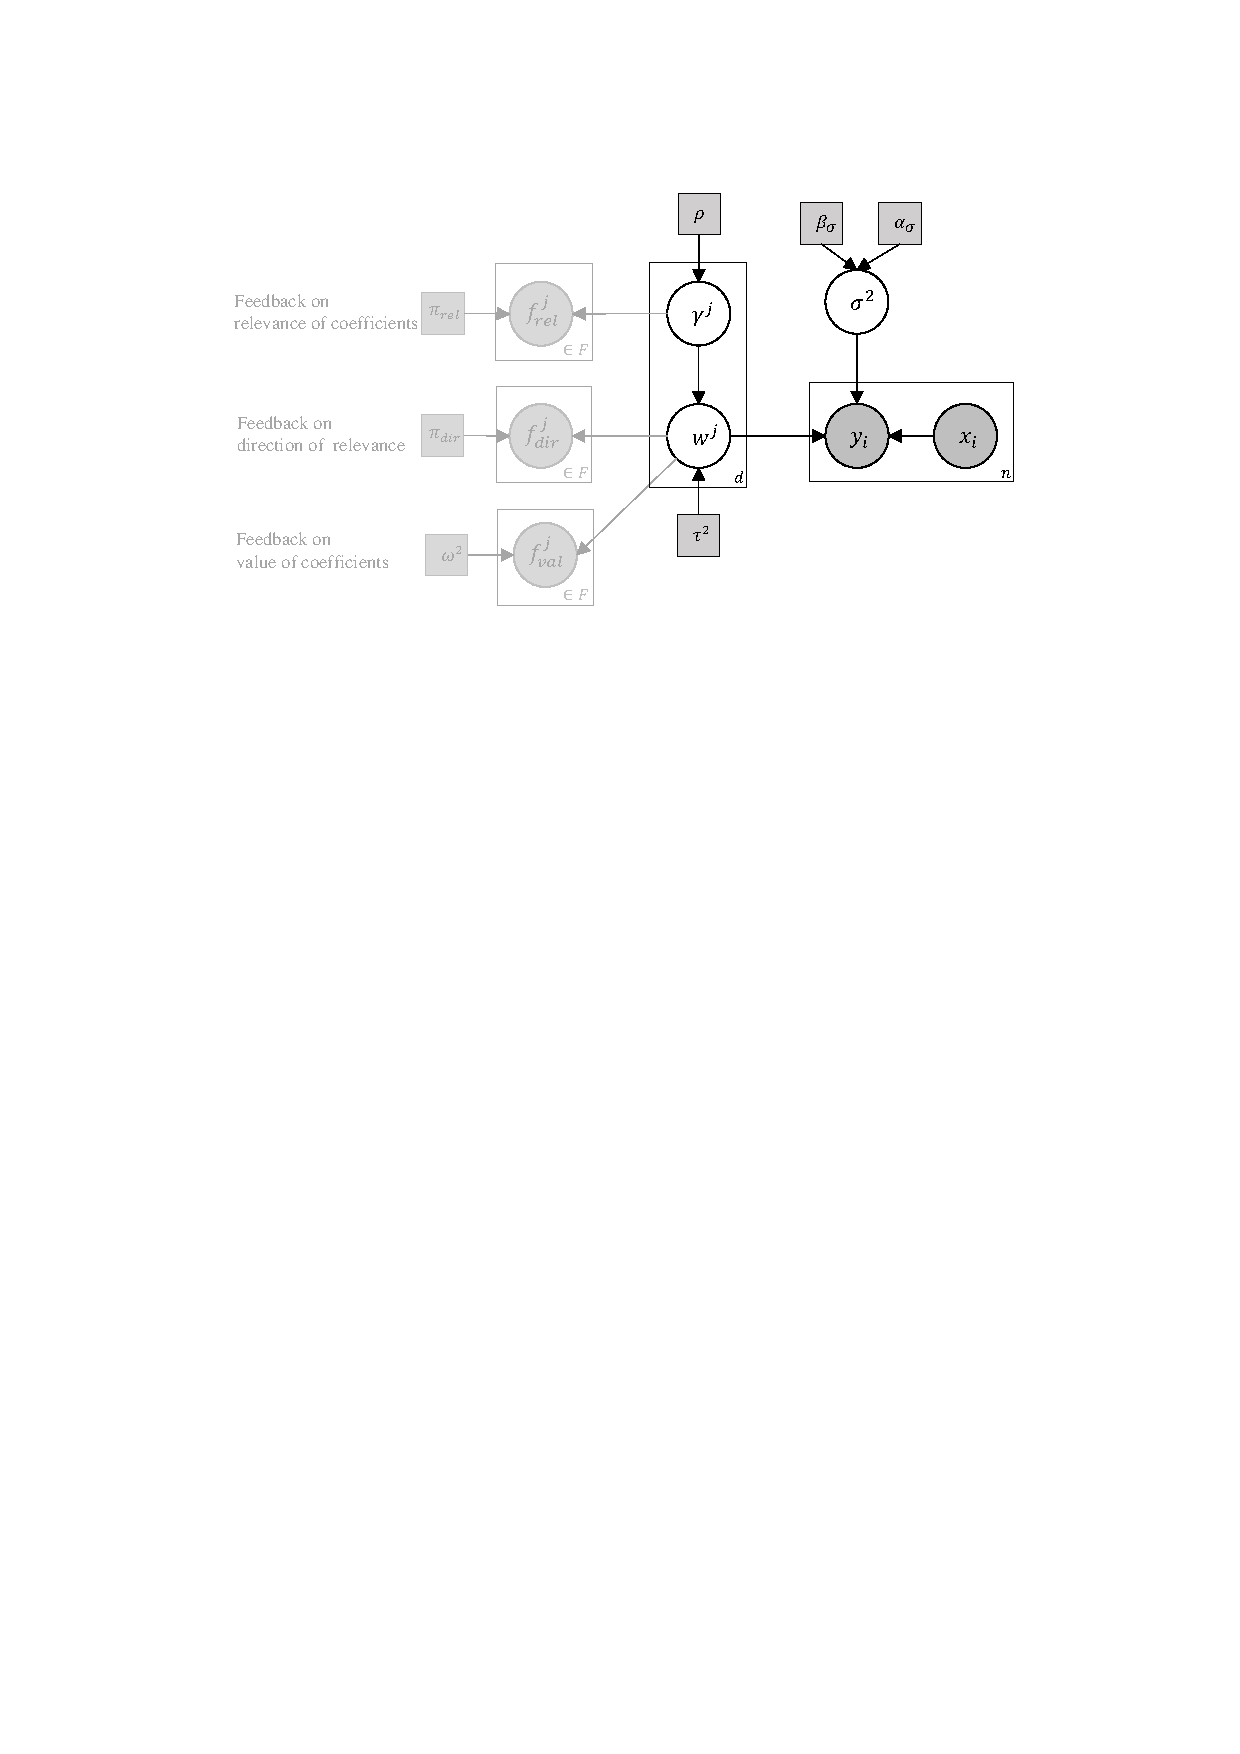
\includegraphics[width=\linewidth]{Figures/Plate_diagram_KE.pdf}
	\caption{Plate notation of the prediction model (right; see Equation \ref{Eq:ss_Bayesian_regression}) and user feedback observations (left; see Equations \ref{Eq:fb_on_val_coeff}, \ref{Eq:fb_on_rel_coeff}, and \ref{Eq:fb_on_dir_coeff}). User feedback influences the data model through observations about model parameters. Circles represent variables (observed variables are shaded), and shaded squares are the fixed hyperparameters.}
	\label{fig:Plate_KE}
\end{figure}


\begin{itemize}
	\item With some noise, the user can provide feedback about the value of coefficients
	\begin{equation}\label{Eq:fb_on_val_coeff}
	f_{val}^{j} \sim \normalpdf(w^j, \omega^2),
	\end{equation}
	\noindent where $\omega^2$ models the variance of error in user feedback. Knowledge about value of coefficients is very powerful, however, only available in some specific applications (e.g., exploiting similar trained models or reported values in related literature). 
	\item With some probability, the user can provide feedback about whether a coefficient should be included or excluded from the model
	\begin{equation}\label{Eq:fb_on_rel_coeff}
	f_{rel}^{j} \sim \gamma^j \bernoullipdf(\pi_{rel}) + (1 - \gamma^j), \bernoullipdf(1 - \pi_{rel}).
	\end{equation}
	\noindent where $\pi_{rel}$ indicates the probability that user is correct about the feedback. This relevant/not-relevant feedback is the simplest form of knowledge that a user may have about a regression model. 
	\item With some probability, the user can provide feedback about direction of relevance of a coefficient, i.e., whether a feature is positively or negatively correlated with the response variable
	\begin{equation}\label{Eq:fb_on_dir_coeff}
	f_{dir}^{j} \sim I(w^j \geq 0) \bernoullipdf(\pi_{dir}) + I(w^j < 0) \bernoullipdf(1 - \pi_{dir}),
	\end{equation}
	\noindent where $\pi_{dir}$ indicates the probability that user is correct about the feedback.
\end{itemize}



The connection of the three mentioned feedback with the data model (Equation \ref{Eq:ss_Bayesian_regression}) is shown as a plate diagram in Figure \ref{fig:Plate_KE}. The full posterior of the unknown parameters given data observations and the user feedback can be described as 

\begin{equation}\label{Eq:Bayes_rule_ss_reg_with_fb}
p(\bw, \bm{\gamma}, \sigma^2 \mid \bD,\bF) = \frac{p(\bD \mid \bw, \sigma^2)p(F_{val} \mid \bw)p(F_{rel} \mid \bm{\gamma})p(F_{dir} \mid \bw)p(\bw \mid \bm{\gamma})p(\sigma^2)p(\bm{\gamma})}{p(\bD,\bF)},
\end{equation} 

\noindent where $F_{val}$, $F_{rel}$, and $F_{dir}$ are the sets of collected feedback corresponding to the three considered feedback types and $\bF = (F_{val}, F_{rel}, F_{dir})$. The posterior computation is discussed in Section \ref{posteriro_inf}.

%It should be noted that there is no restriction on the amount of feedback (or the types) available for computation of the posterior. 



\subsubsection{Related works}

The proposed feedback models provide an intuitive and effortless way for the user to directly influence the prediction model without caring about the complications of the data model. Classical prior elicitation (see for example \cite{OHagan06,garthwaite2005statistical}) aims at eliciting a distribution to represent the expert's knowledge by asking about summary information such as quantiles of the parameters. This is done through iterations between the expert in the related field and statisticians who design the model. Our work goes beyond pure elicitation as it directly connects the expert to the model and also exploits the training data to facilitate the interaction as will be discussed more in Section \ref{interaction}.

We have considered three intuitive types of feedback models. Studies have shown that the type of domain knowledge in prediction tasks can be summarize in a small set \cite{concept_driven_CHI2019}. A large body of works have studied the exclusion/inclusion of features (also known as feature selection \cite{Correia2019HumanintheLoopFS}) in different contexts, for classification  \cite{raghavan2006active,druck2009active,settles2011closing}, and regression \cite{Micallef_elicitation}. These methods are different to ours from the modelling point as we consider sparse models and also the type of interaction. A different type of feedback is the case where user has knowledge about pairwise similarity of features with respect to the response variable (i.e., asking the user about which  pairs of features affect the prediction output similarly) which has been investigated in \cite{Homayun_pairwise_UMAP,Homayun_pairwise_ijcai2019}.  

\subsection{User feedback as outcome of a cognitive process}

The feedback models proposed in the previous section consider the user as a passive data provider with some noise models. However, humans are more complicated than that. Publication IV investigates a similar knowledge elicitation task to the previous section, but aims at accounting for rational process that humans may undergo to produce the feedback during the interaction. In other words, we will define a more complex feedback model that accounts for the cognitive process of the user, with the idea that performance can be improved if we also model the thought process behind the feedback.

\begin{figure}
	\centering
	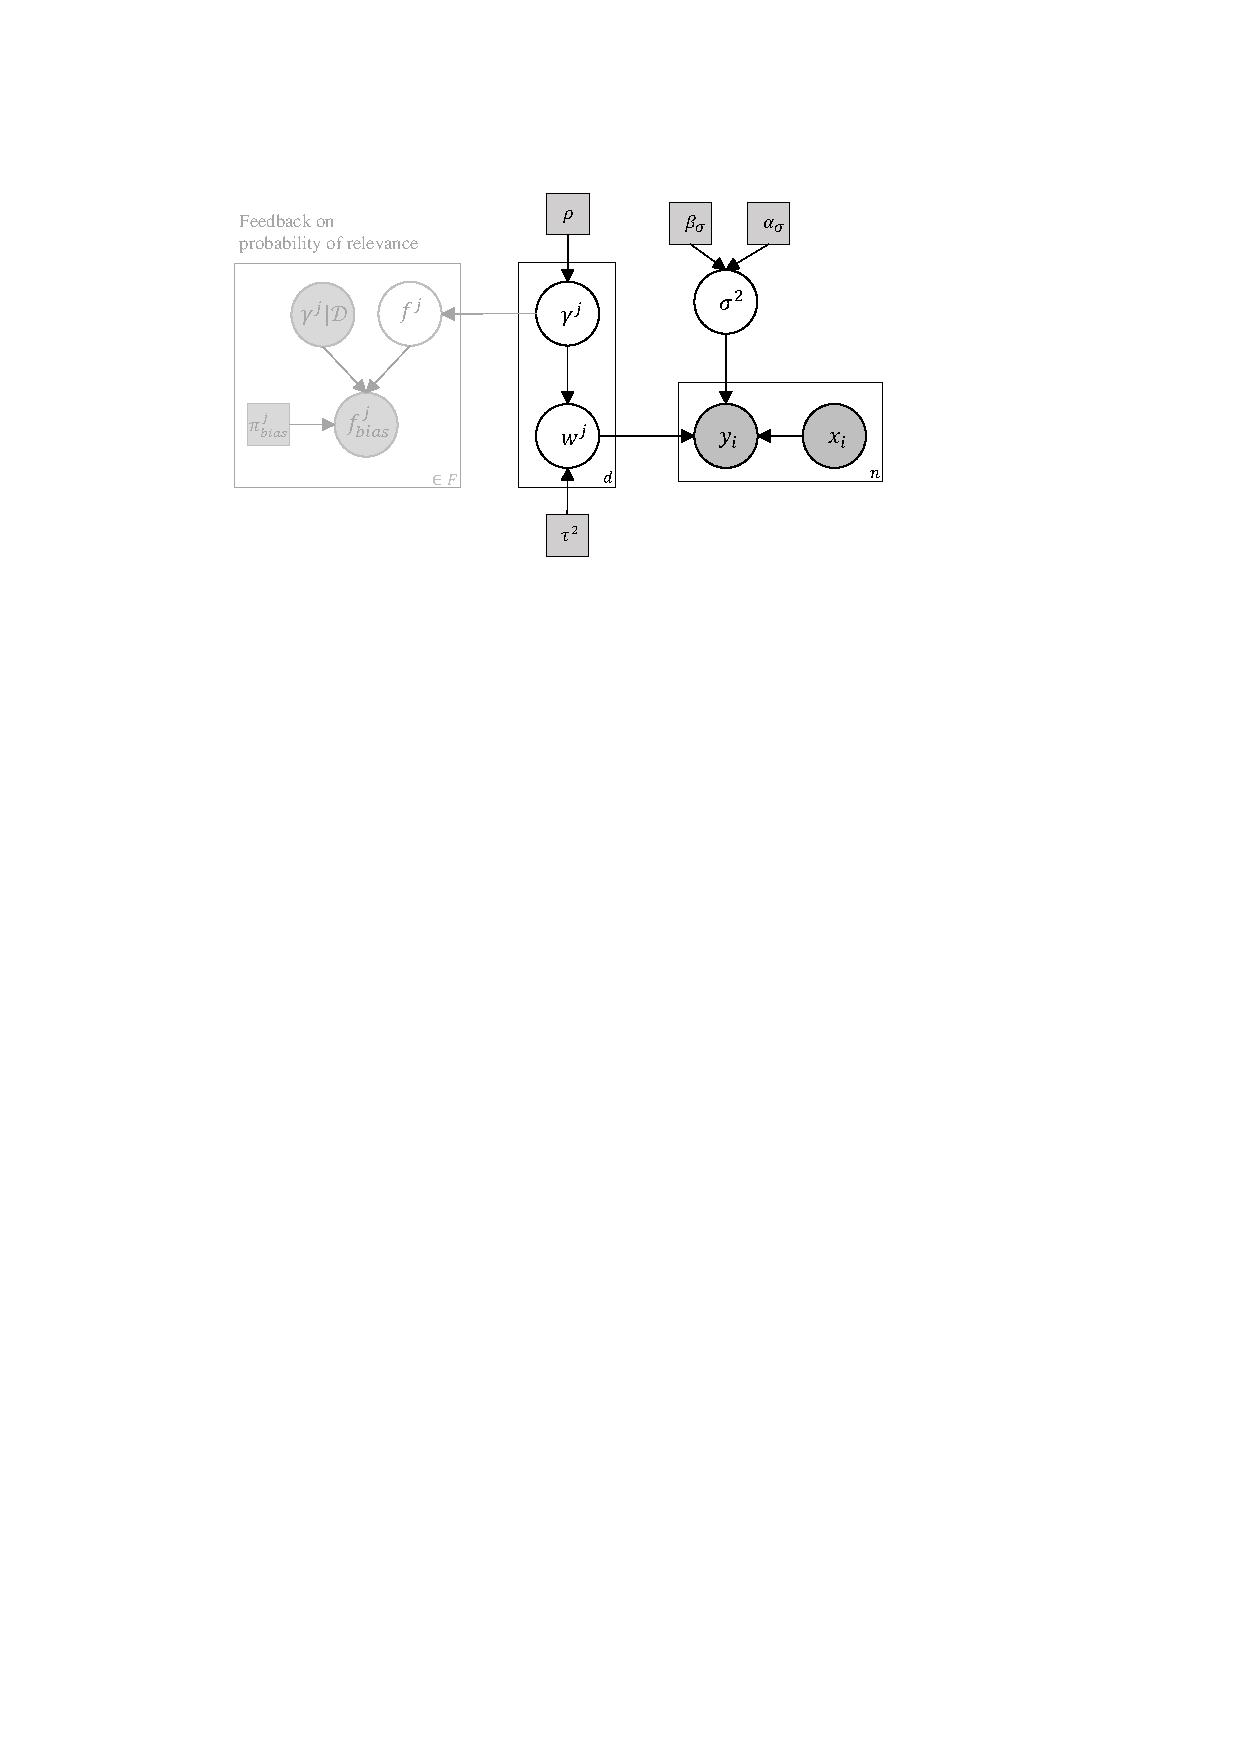
\includegraphics[width=0.80\linewidth]{Figures/Plate_diagram_OF.pdf}
	\caption{Plate notation of the prediction model (right; see Equation \ref{Eq:ss_Bayesian_regression}) and user model for feedback (left). The observed user feedback about the probability of relevance of coefficient, $p(\gamma^j \mid \bD,f^j)$, is biased as it is generated from combination of latent user knowledge about the coefficient, i.e., $p(f^j \mid \gamma^j)$, and information visualized from the data model about probability of relevance of the coefficient, i.e., $p(\gamma^j\mid \bD)$. We are interested in inferring the unbiased, latent, version of the feedback to update the parameters of interest in the data model.}
	\label{fig:Plate_OF}
\end{figure}

In many interaction scenarios, such as visual analytics or human in the loop machine learning systems, certain aspects of the training data, such as statistics or outputs of the machine learning method, may be revealed to the user  \cite{BEAMES_Endert,sacha2017you,Homayun_pairwise_UMAP,muhlbacher2013partition,Talbot2009,van2011baobabview,Kapoor2010,krause2014infuse,sarkar2015interactive,Micallef_elicitation}. This is mainly done to provide information about important characteristic of the data to improve decision making or to guide the user to facilitate the interaction. For example, in the mentioned knowledge elicitation tasks, the system may first show what it has learned about the coefficient of the linear model from the training data and then ask for the user feedback about the same coefficient. Though very common, this type of interaction is prone to overfitting, as the user feedback may not be independent of the knowledge in the training data, while the machine learning methods commonly assume independence between data and user input. Studies in cognitive science have shown that humans are unintentionally biased toward the pieces of information provided for them \cite{Tversky1974,garthwaite2005statistical}. We propose a user model that accounts for such bias. In other words, the user model assumes that the user is rational \cite{gershman2015computational} and combines the information provided to her with her knowledge and then provides feedback as the outcome of such cognitive procedure. The user model can then undo the bias in the feedback by performing the inverse of the same rational update.

In particular, we consider the case where the user provides feedback about the probability of relevance of a coefficient. %This new feedback type can be modelled by \ref{Eq:fb_on_rel_coeff} with the difference that both $f_{rel}^{j}$ and $\pi_{rel}^{j}$ are jointly observed as feedback for the $j^{th}$ feature (e.g., the user input  $f_{rel}^{j}=1$ and $\pi_{rel}^{j}=0.8$ describes the user belief that the probability of relevance of the $j^{th}$ feature is $0.8$).
The belief of the model (based on data alone) about the probability of relevance of the coefficient, i.e., marginal posterior probability $p(\gamma^j \mid \bD)$, is also visualized for the user. We make the assumption that the user is rational in first combining the visualized information from data with her latent knowledge. The reported feedback is the updated knowledge which is naturally biased as it is partially coming from information in the training data. The model should consider this while inferring the posterior of the parameters of interest given the user feedback. Figure \ref{fig:Plate_OF} depicts a schematic of the data and user feedback model for this problem.% (note that we renamed the observed feedback to $f_{bias}^{j}$ and $\pi_{bias}^{j}$).
 
We assume that the user is rational and combines her latent knowledge about the probability of relevance of the $j^{th}$ coefficient, i.e., $p(f^{j} \mid \gamma^j=1)$, with the revealed information from the training data, i.e., $p(\gamma^j =1 \mid \bD)$, following a Bayesian update

\begin{equation}\label{Eq:Bayesian_update_biased_fb}
p(\gamma^j=1 \mid \bD, f^{j}) \propto p(f^{j}\mid \gamma^j=1)p(\gamma^j =1\mid \bD),
\end{equation}  

\noindent and provides as feedback the resulting posterior  $p(\gamma^j=1 \mid \bD, f^{j})$. The latent feedback likelihood can be represented as $p(f^{j}\mid \gamma^j) = \pi^j \gamma^j + (1-\pi^j) (1-\gamma^j)$, with $\pi^j$ being the likelihood for latent feedback when $\gamma^j=1$. By doing the reverse of the Bayesian update in \ref{Eq:Bayesian_update_biased_fb}, we can infer $\pi^j$ as:

\begin{equation}\label{Eq:latent_knowledge_infer}
\pi^j \propto \dfrac{p(\gamma^j=1 \mid \bD, f^{j})}{p(\gamma^j =1\mid \bD)}.
\end{equation}  

We can then use the inferred user feedback $p(f^{j}\mid \gamma^j)$, instead of the observed one, to update the posterior for the parameters of interest. Publication IV shows in a simple user study that the prediction performance in a simple sentiment analysis task can be improved if the user model accounts for the rational updates that the user may undergo.

\subsubsection{Related works}

Human bias in interactive tools has been discussed in prior elicitation \cite{garthwaite2005statistical}, and visual analytics \cite{bias_warning}. In particular, \cite{garthwaite2005statistical} reviews the common human biases from psychological literature and provides guidelines for how to reliably extract expert knowledge about uncertain quantities. \cite{bias_warning} proposed a framework for measurement of such biases in visual analytics tools and investigated how to overcome it through informing the user of potential biases. Our work is fundamentally different as we are not limiting or interrupting the interaction (by just following a guideline or showing a warning), but rather, acknowledge the presence of such biases and allow the user model, as part of the system, to account for that.

%HAVE OTHERS TRIED TO INFER MODE FROM THE USER? MAYBE CITE OUR NEURIPS PAPER AND SOME RL. DO NOT CITE APPLICATIONS HERE.
%Several works have investigated methods to extract more from the user feedback alone. Maybe RL works? Our work, is the first to 


\subsection{User feedback for intent modelling} 
% The problem here is that the work here cannot be generalized to other applications. I need to introduce documents and keywords!
Intent modelling describes the task of learning the hidden intent of the user from user feedbacks. Unlike the previous mentioned scenarios where the user feedback was used as complementary information to the training data, in Publication I and V the task is to predict the user intent based on user feedback alone. An important instance of this scenario is the interactive personalized search systems where in each iteration the system recommends items and the user provides feedback regarding relevance of recommendations. The goal is not just to better predict relevance of items for the user but rather to find the most relevant item with minimal interaction. In this section, we discuss the probabilistic modelling of this task and later in Section \ref{interaction} discuss how to design the interaction so that the most relevant item can be learned as fast as possible. 

Consider the case where a user is searching for a scientific article by forming a query with keywords. The user is uncertain about the exact description of the article (e.g., the user may not know the tile), however, if the article is recommended, the user can assess the relevance of it. This information seeking task is usually done in several iterations starting with an initial query, assessing the results recommended by the system, and modifying the query with the goal of getting better results. This type of information seeking with the user being uncertain about her information need, is known as exploratory search \cite{Marchionini2006,white2009exploratory} and covers around half of search behaviours of users \cite{Teevan_2004} (see \cite{paba_exploratory_vs_lookup} for more in depth review for exploratory and standard lookup search). The main bottle necks of such search systems are that (i) the amount of user feedback that can be gathered is very limited compared to the size of the information space, and (ii) the users are mostly sometimes reluctant to give more than few explicit feedback after assessing the recommended results. To tackle these challenges, Publication I, exploits the relationship between articles and their keywords and defines feedback likelihoods on both keywords and articles, providing more flexibility for the user to express its intent. Furthermore, the modelling of noisy implicit feedback, in particular feedback generated from brain activity measured through electroencephalography (EEG) and eye movements, is investigated in Publication V.  

The intent model is defined as function that maps all the keywords (used to express the search intent) and articles to real values, indicating the relevance of each item for the user. As the number of user feedback is few, it is reasonable to use a linear model to define the relation of user feedback on keywords to the hidden intent (denoted by $\bw$)

\begin{align}\label{Eq:feedback_on_kw} 
f_{kw}^{i} \sim \normalpdf(\bm{x}_i\tp \bw, \sigma_{kw}^2), 
\end{align}

\noindent where $\sigma_{kw}^2$ models the noise of the keyword feedback. The keywords are represented in the keyword-document matrix $X \in \mathbb{R}^{k \times d}$ where the element $(i,j)$ describes the tf-idf weighting of keyword $i$ (out of $k$ total keywords) in document $j$ (out of $d$ total documents), and $\bm{x}_i\tp$ indicates the $i^{th}$ row of the matrix. As mentioned, we are interested to also model potential user feedback on the documents. We make the simplifying assumption that the expected relevance of a document can be represented as a weighted sum of the expected relevance of keywords that appear in it

\begin{align}\label{Eq:doc_key_relation} 
 \E[f_{doc}^{j}] = \sum_{i=1}^{k} p_{(i \mid j)}  \E[f_{kw}^{i}],
\end{align}

\noindent where $f_{doc}^{j}$ indicates the relevance of the $j^{th}$ documents, $\E[.]$ denotes the expected value and $p_{(i \mid j)}$ is the likelihood of the $i^{th}$ keyword being present in the $j^{th}$ document. This likelihood is not available but can approximated by normalizing $X$ such that its columns sum up to one. Denoting the resulting matrix as $\hat{X}$ and following following \ref{Eq:feedback_on_kw}, the feedback for relevance of documents can be described as 

\begin{align}\label{Eq:doc_key_relation_vector} 
F_{doc} \sim \normalpdf(  \hat{X}\tp X \bw, \sigma_{doc}^2 \eye),
\end{align}  

\noindent where $F_{doc}=[f_{doc}^{1},\ldots,f_{doc}^{d}]$ is the vector representation of relevance feedback for all documents, and $\sigma_{doc}^2$ models the noise of the document feedback. 

Given user feedback on keywords and documents the posterior of the hidden intent can be learned by assuming a Gaussian prior on the intent weights, i.e., $\bw \sim \normalpdf(0,\tau^2 \eye)$. As the both likelihoods follow a Gaussian distribution, the posterior has a closed form solution and can be derived following the same derivations as the simple linear model in \ref{Eq:lin_rel_simple_posterior}. Figure \ref{fig:Plate_intent_kd} illustrates the schematic of user feedback models and its connection to the latent intent. 


\begin{figure}
	\centering
	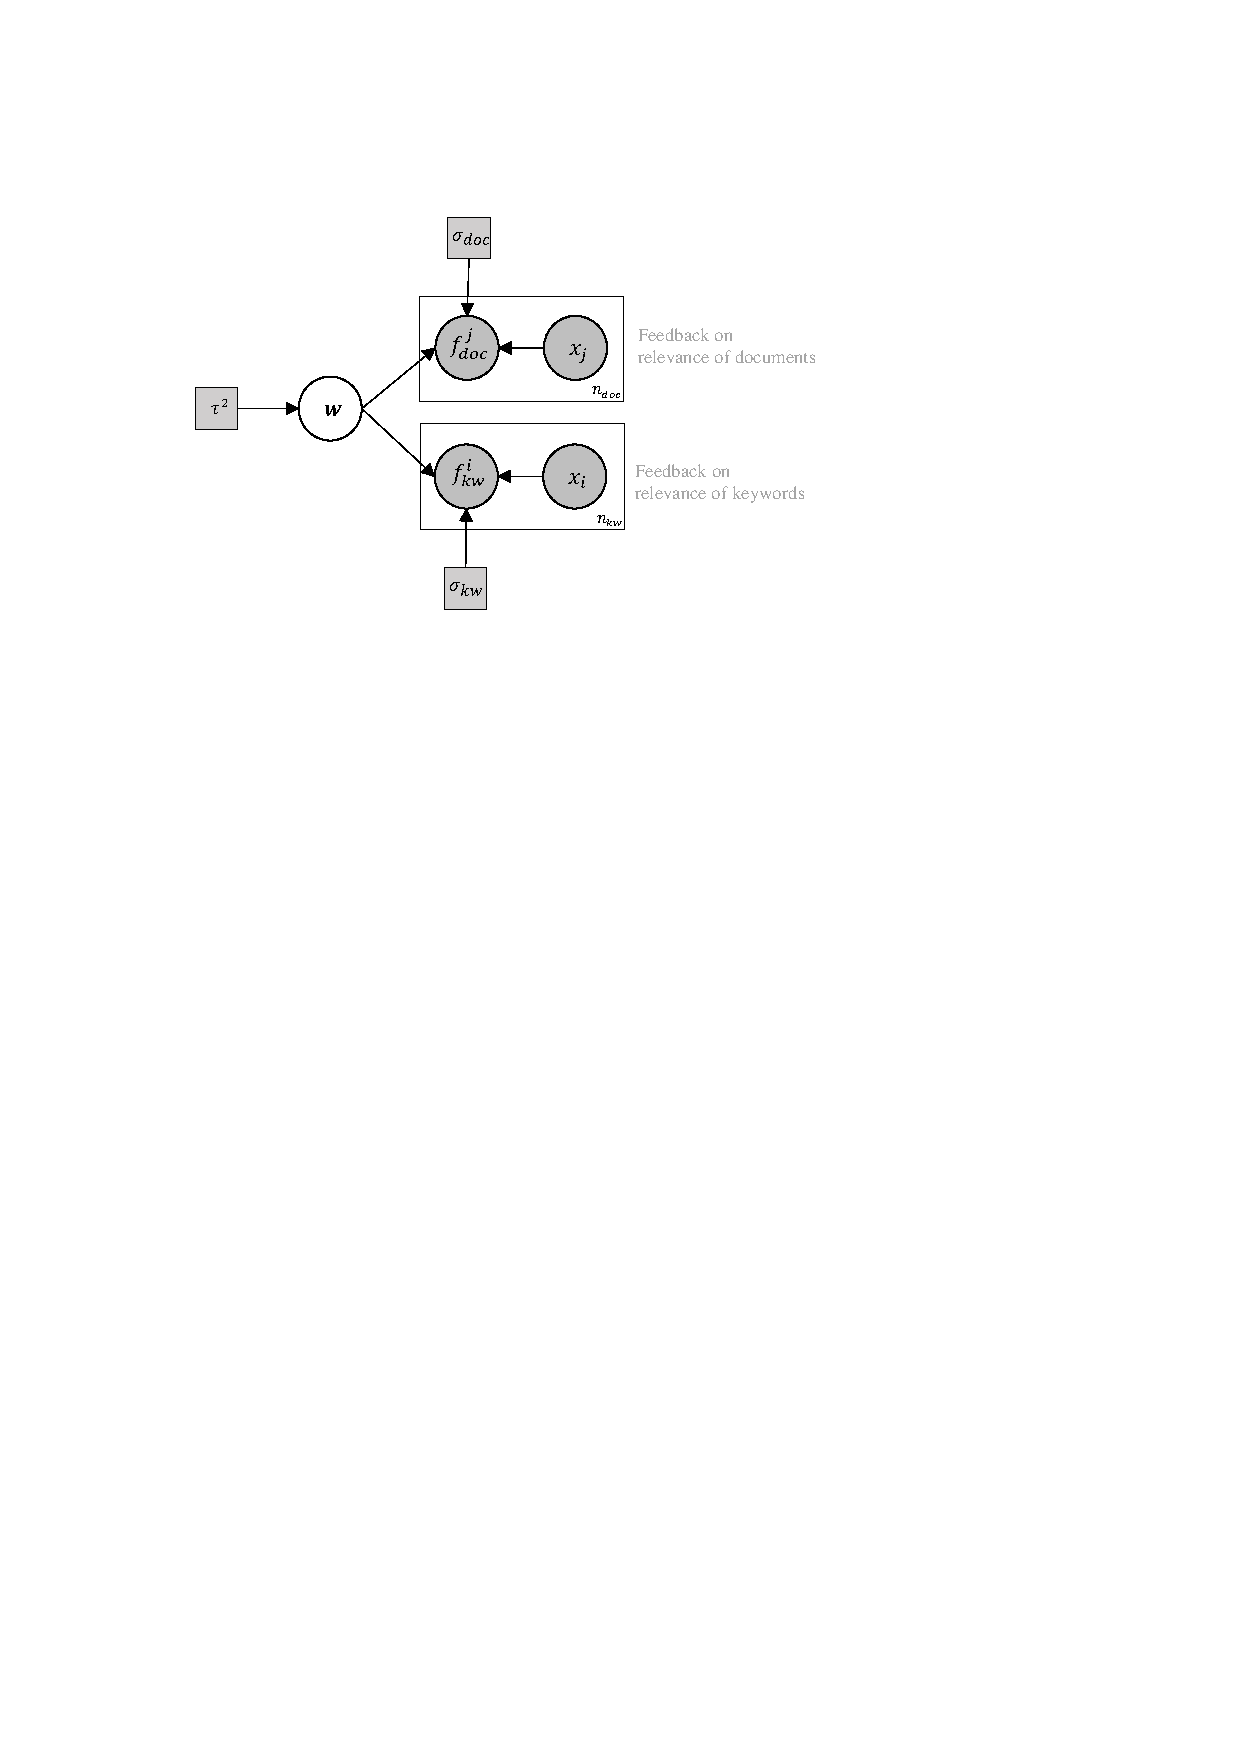
\includegraphics[width=0.80\linewidth]{Figures/Plate_diagram_intent_kd.pdf}
	\caption{Plate notation of the intent modelling from feedback on recommended documents and keywords. The feature transformation are now shown. The feature for the $i^{th}$ keyword (shown as $x_i$) is the $i^{th}$ row of keyword document matrix $X$, and for the $j^{th}$ document (shown as $x_j$) is the $j^{th}$ column of $\hat{X}\tp X$.}
	\label{fig:Plate_intent_kd}
\end{figure}


\subsubsection{Implicit feedback model}

The model proposed model is very simple as the noise of feedback is assumed to be known and the only unknown parameter is the intent vector $\bw$. As mentioned, we are interested to consider feedbacks from implicit sources such as neurophysiologic signals gathered from brain activities\footnote{Note that here we assume that the implicit feedbacks, EEG signals, are already converted to a continuous relevance value (see Publication V for details about this conversion).}. The implicit feedback is extremely cheap, as the it requires no physical effort from the user, but at the same time extremely noisy. Our modelling solution is to use the automatic relevance detection model proposed in \ref{Eq:ard_Bayesian_regression} to endow the feedback likelihood handle the inherent noise in the implicit feedback when used in combination of the explicit feedbacks. For simplicity, let's assume that only the keyword feedback is generated from an implicit source (it is straightforward to consider a similar feedback source for documents or to consider both explicit and implicit feedback for keywords or documents). The implicit feedback likelihood for keywords can be expressed as 

\begin{align}\label{Eq:imp_fb_on_kw} 
f_{kw}^{i} \sim \normalpdf(\bm{x}_i\tp\bw,\frac{\sigma_{kw}^2}{\nu_i}),
\end{align}  

\noindent where the parameters follow the model \ref{Eq:ard_Bayesian_regression}. The model can then infer the accuracy of feedback $\nu_i$ based on the observed feedback and handle the high uncertainty in implicit feedback. The resulting model for a case of availability of explicit feedback on documents and implicit feedback on keywords is depicted in Figure \ref{fig:Plate_intent_imp}. The resulting posterior is analytically intractable.  

\begin{figure}
	\centering
	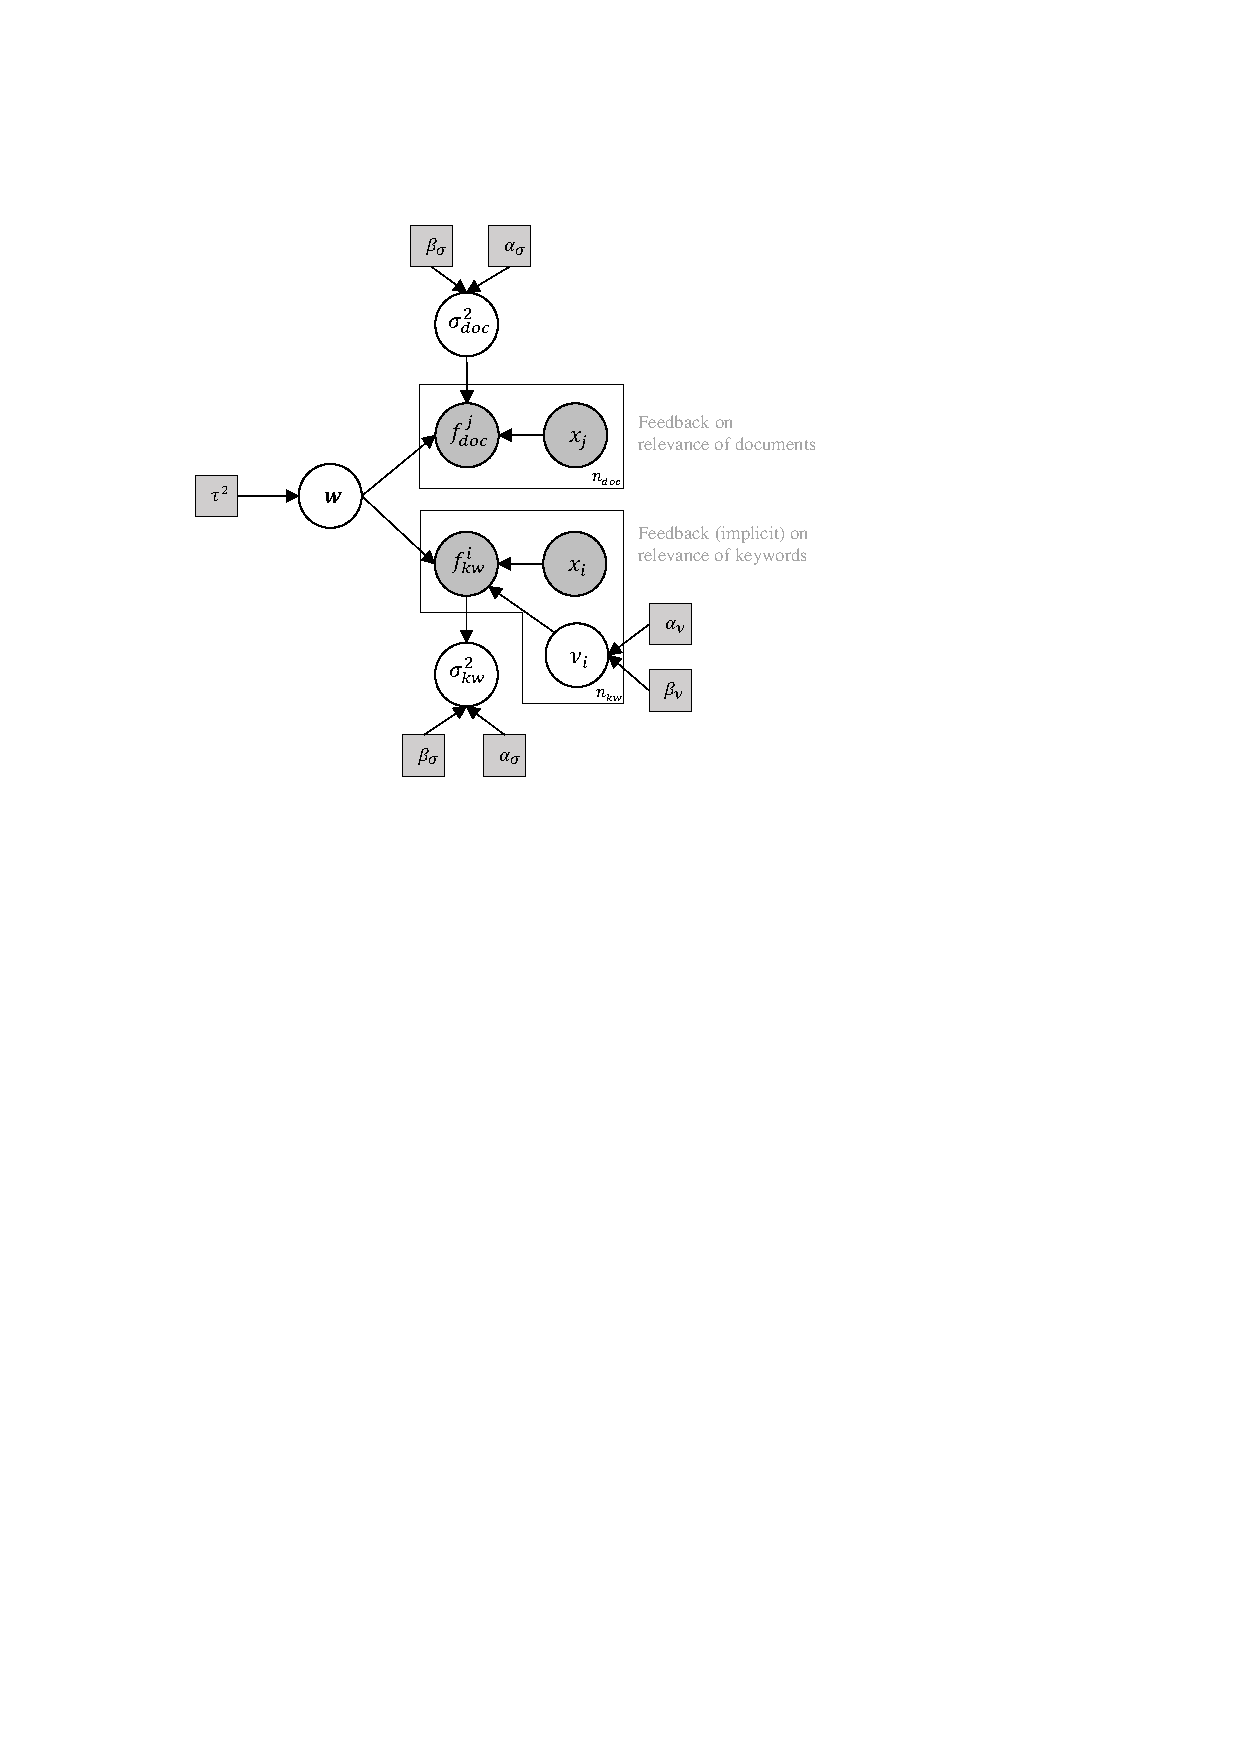
\includegraphics[width=0.80\linewidth]{Figures/Plate_diagram_intent_imp.pdf}
	\caption{Plate notation of the intent modelling from feedback on recommended documents and noisy, implicit feedback on keywords. The data model is based on \ref{Eq:ard_Bayesian_regression} with the feedbacks as the observational data. The feature vector of documents follows the transformation introduced in equation \ref{Eq:doc_key_relation_vector}}
	\label{fig:Plate_intent_imp}
\end{figure}

   
\subsubsection{Related works}
Intent modelling for article search has been studied in  \cite{GlowIUI2013,ruotsalo2015interactive,Ruotsalo2018}. These works are different to ours as they only define the intent on keywords and then use the learned intent as an input to a separate retrieval model (based on a standard language model) to retrieve ranked documents, while document retrieval is a natural outcome of the document feedback likelihood in our work. Furthermore, the previous methods did not consider the option of user providing feedback on documents. We borrowed the same user interface for providing feedback on keywords which is based on the idea of visualizing the top relevant keywords in a radar-like interface where the distance to center for each keyword is proportional to the predicted relevance from the intent model. The user then can provide feedback by dragging a keyword toward the center (indicating positive relevance) or further away from the center (indicating negative feedback). We added document feedback through clicks or bookmarking. 



\section{Posterior inference} \label{posteriro_inf}
Other than simple models (like the linear regression introduced in \ref{Eq:lin_rel_simple_posterior}) the models proposed in this thesis do not have a closed-form posterior and posterior predictive distributions. For low dimensional unknown parameters, it is still practical to approximate the posterior distribution by simulation methods such as numerical computation on girds or Monte Carlo simulations (see \cite[Chapter~10]{Gelman2013} for a review). However, as mentioned, we are interested on high-dimensional problems (e.g., sentiment analysis and search with textual data, or drug response prediction with genomic data), where simple simulation methods cannot scale well due to the curse of dimensionality (the number of evaluations grows exponentially with respect to the dimension). There are two general family of methods to approach such intractable posteriors --namely Markov chain simulation and deterministic posterior approximation methods.

\subsubsection{Markov chain simulation methods}

Markov chain simulation methods are general methods to draw samples from the target posterior, i.e., $\theta^s \sim p(\theta \mid \bD)$, by starting from an initial sample in the parameter space and sequentially updating the sample toward the target posterior distribution. The sequence of dependent samples forms a chain which should have the Markov property, i.e., the updating rule to get to $\theta^{t+1}$ at time $t+1$ should only depend on the previous sample $\theta^t$, and not the whole chain. It can be shown that under some assumptions for the updating rule and the Markov chain, by increasing the chain size toward infinity, the last sample in the chain would be a sample from the target distribution \cite[Chapter~11]{Gelman2013}. Recent advances in Markov chain simulation methods has resulted in probabilistic programming languages, such as Stan \cite{STAN} and Pyro \cite{bingham2018pyro}, that make the computation of Bayesian inference straightforward for end users. The user of such softwares needs to declare the model, and the probabilistic programming language performs the inference by providing samples from the posterior (for example see \cite{Bayesian_workflow_cog_sci_2019} for a step-by-step guides to do Bayesian modelling and inference using Stan). The posterior samples can be used to compute predictive distributions, summaries (such as expected value or other estimates), or utilities for decision making. A bottleneck of iterative simulation methods is that they can sometimes be slow. This is particularly important in the works investigated in this thesis as all of them require real-time performance with a user.

\subsubsection{Deterministic posterior approximation}

The idea of deterministic approximation methods is to approximate the target distribution, such as posterior distribution $p(\theta \mid \bD)$, with a simpler distribution $q(\theta)$ (e.g., from exponential family), i.e., $q(\theta) \approx p(\theta \mid \bD)$. The resulting approximation does not fully represent the target distribution, however, in many cases it can be efficient or accurate enough for the targeted task. There are different ways, e.g., different objective functions or assumptions about the approximated distribution, to handle the approximation. Here we briefly review some of the common methods that have been also employed in this thesis. 

\begin{itemize}
	\item Expectation propagation (EP) \cite{minka2001expectation} aims at finding $q(\theta)$ that minimizes the Kullback–Leibler ($\KLt$) divergence between the posterior and the approximation, i.e., $\KL{p(\theta \mid \bD)}{q(\theta)}$. KL-divergence is a popular asymmetric measure of how two distributions are different from each other. The minimization is usually intractable. The posterior distribution can be written as a product of terms $p(\theta \mid \bD) = \prod_{j} t_j(\theta)$ (for example the posterior in \ref{Eq:Bayes_rule_ss_reg_with_fb} is a product of seven terms). It it is sensible to consider the same structure for the approximated posterior $q(\theta) = \prod_{j} \tilde{t}_j(\theta)$. % \dfrac{1}{Z}, where $Z$ is a normalization factor. 
	EP approximates each term $t_j(\theta)$ in the posterior by a simpler exponential family form $\tilde{t}_j(\theta)$ such that $\prod_{j} t_j(\theta) \approx \prod_{j}\tilde{t}_j(\theta)$. As the exponential family is closed under product, $q(\theta)$ also follows a simple and tractable exponential form. To optimize the terms, EP iteratively refines the parameters of $\tilde{t}_j(\theta)$ to minimize $\KL{t_j(\theta) q^{\!\!\!\backslash j}(\theta)} {\tilde{t}_j(\theta) q^{\!\!\!\backslash j}(\theta)}$, where $q^{\!\!\!\backslash j}(\theta)$ denotes the approximated posterior after removing the $j^{th}$ term, i.e.,  $q^{\!\!\!\backslash j}(\theta) \propto \frac{q(\theta)}{\tilde{t}_j(\theta)}$. This is optimized by matching the sufficient statistics of $t_j(\theta) q^{\!\!\!\backslash j}(\theta)$ with $\tilde{t}_j(\theta) q^{\!\!\!\backslash j}(\theta)$. After refining each $\tilde{t}_j(\theta)$, an updated approximation is achieved as $q(\theta)\propto q^{\!\!\!\backslash j}(\theta) \tilde{t}_j(\theta)$. This step is repeated until all the terms converge.  \cite{hernandez2013generalized,Lobato2015ML,Tomi_P_thesis}
	
	EP can provide good estimate to uncertainty (e.g., approximation for the posterior covariance of the weights in the linear model) that is desirable for designing the interaction (experimental design methods; see Section \ref{AL_and_ED}) \cite{hernandez2013generalized}. Furthermore, for sequential interaction, the inference can be sped up by only performing few iterations of parameter updates (instead of waiting for full convergence) as suggested by \cite{seeger2008bayesian}. EP was used in Publication II and III for fast approximation of the posterior of the linear regression model with sparsity-inducing spike-and-slab prior on coefficients with data and feedback observations (Equation \ref{Eq:Bayes_rule_ss_reg_with_fb}). The regression weights ($\bw$) are approximated by a multivariate Gaussian distribution. 
	
	\item Variational Bayesian (VB) methods aim at minimizing $\KL{q(\theta)}{p(\theta \mid \bD)}$ (unlike EP).
	
	\item Normal (Laplace) approximation where the posterior is approximated with multivariate normal distribution (see \cite[Chapter~4]{Gelman2013} for a review), 
	
 
\end{itemize}

\section{Key components of the joint model}\label{key_comp}



%\item Idea: Have a picture per section where there is a cloud on top of user and system head and in it there is the plate diagram of the particular model. Then talk about the interaction. 
%In the first introduction section have the same figure but just write down (or explain) user probabilistic model and data probabilistic model (priors) and arrows for interactions? and then refer to later chapters for the type of interaction

%\item Then explain the two possible likelihoods and show a diagram where there is a section for data modeling and there is a section for user modeling that are connected through a shared latent parameter and then each have their own models. Then explain that we will go through details of the data and user model in the next two subsections. My contribution comes from adding data likelihoods and user priors and having interaction.

%I design probabilistic machine learning models to tie the data model (prediction model from the training data) to the user model (the model of the human) in a unified way. After doing so, we use Bayesian inference to find the posterior, i.e, distribution of the unknown parameters related to data and user, giving the training data and user interaction. The posterior inference, in most cases, does not have an analytical solution. We use different approximation methods, such as expectation propagation and variational inference, to handle the computation.


\textcolor{red}{Let $y$ and $x$ denote the outputs (target variables) and inputs (covariates), and $\theta$ and $\phi_y$ the model parameters. Let $f$ encode input (\textit{feedback}) from the user, presumably a domain expert, and $\phi_f$ be model parameters related to the user input. We identify the following key components:
	%
	\begin{enumerate}%[leftmargin=*,noitemsep,topsep=0pt]
		\item An observation model $p(y\mid x,\theta,\phi_y)$ for $y$. %data model
		\item A feedback model $p(f\mid\theta, \phi_f)$ for the expert's knowledge. % user model
		\item A prior model $p(\theta, \phi_y, \phi_f)$ completing the hierarchical model description.
		\item A query algorithm and user interface that facilitate gathering $f$ iteratively from the expert.
		\item Update process of the model after user interaction.
	\end{enumerate}
	%
	The observation model can be any appropriate probability model. It is assumed that there is some parameter $\theta$, possibly high-dimensional, that the expert has knowledge about. The expert's knowledge is encoded as (possibly partial) feedback $f$ that is transformed into information about $\theta$ via the feedback model. Of course, there could be a more complex hierarchy tying the observation and feedback models, and the feedback model can also be used to model more user-centric issues, such as the quality of or uncertainty in the knowledge or user's interests.}



TO EXPLAIN: Why we use linear models? because of the risk for overfitting if the model is not regularized enough... and also mentioning what model was used in each publication?

\chapter{User interaction with the probabilistic model}\label{interaction}

%Here have the same figure, explain how user feedback is gathered. explain that we consider two sets of works. One where there is external data other than user feedback and one where the user feedback IS the data. Then explain our interaction goals and acquisition functions and experimental design.

\section{Active learning and experimental design}\label{AL_and_ED}

\section{Multi-armed bandits and Bayesian optimization}

\chapter{Summary of the Contributions}
%Applications and results OR Summary of the Publications
%Go through the papers and tasks. 
This chapter briefly summarizes the contributions of Publications I-V with emphasize on answering the research questions of the thesis. 

\section{Interactive intent modelling from multiple feedback domains (Publications I and V)}

\section{Expert knowledge elicitation for high-dimensional prediction (Publications II and III)}

\section{User modelling for avoiding overfitting in knowledge elicitation (Publication IV)}


\chapter{Discussion}


%Motivate future works such as next level of user modelling. Similar to overfitting work, but assuming a more active version of the user -> ATOM





%--------------------------------END--------------------------%


 % Refer to the Journal paper 1 of this example document
%\citepub{j1} \& \cpub{j1} \& \cp{j1} \& \pageref{j1} \& \ref{j1}
% Refer to the Conference paper of this example document
%\citepub[p.~2]{c1} \& \cpub[Sec.~ 1]{c1} \&  \cp[pp.~1--2]{c1} \& \pageref{c1} \& \ref{c1} 


\renewcommand{\bibname}{References}
\bibliographystyle{plain} % Change as required
\LARGE\bibliography{references}  % remember to edit the file name




%% The following commands are for article dissertations, remove them if you write a monograph dissertation.

% Errata list, if you have errors in the publications.
%\errata

%% The first publication (journal article)
% Set the publication information.
% This command musts to be the first!
\addpublication[conference]{\underline{Pedram Daee}, Joel Pyykk\"o, Dorota G\l{}owacka, and Samuel Kaski}{Interactive Intent Modeling from Multiple Feedback Domains}{Proceedings of the 21st International Conference on Intelligent User Interfaces}{Sonoma, California, USA, 71--75}{March}{2016}{ACM}{c1}

%\addpublication{Journal Paper Authors}{Journal Paper Title}{Journal Name}{Volume, issue, pages, and other detailed information}{Month}{Year}{Copyright Holder}{j1}
%\addpublication[conference]{Conference Paper Authors}{Conference Paper Title}{Conference Name}{Location, pages, and other detailed information}{Month}{Year}{Copyright Holder}{c1}
%\addpublication[accepted]{Journal Paper 2 Authors}{Journal Paper 2 Title}{Journal Name 2}{}{Month}{Year}{Copyright Holder}{j2}
%\addpublication[submitted]{Journal Paper 3 Authors}{Journal Paper 3 Title}{Journal Name 3}{}{Submission date}{Year}{No copyright holder at this moment}{j3}
% Add the dissertation author's contribution to that publication (the order can be interchanged with \adderrata).
\addcontribution{The author had the main responsiblity in problem formulation and modeling. The author designed and implemented the simulation experiment. Joel Pyykk\"o and the author built the system for user studies and conducted them together. The author wrote the initial draft of the manuscript, after which all co-authors joined for revisions.}
% Add the errata of the publication, remove if there are none (the order can be interchanged with \addauthorscontribution).
%\adderrata{j1 I This is wrong}
% Add the publication pdf file, the filename is the parameter (must be the last).
%TODO: uncomment the following in the final version (now commented to increase speed)
%\addpublicationpdf{Articles/IUI16.pdf}



\addpublication[journal]{\underline{Pedram Daee}$^*$, Tomi Peltola$^*$, Marta Soare$^*$, and Samuel Kaski}{Knowledge elicitation via sequential probabilistic inference for high-dimensional prediction}{Machine Learning}{106, 9-10, 1599--1620}{}{2017}{}{j1}
\addcontribution{The ideas and experiments in this article were designed jointly (the first three authors contributed equally). The author had the main responsibility in the derivation of the sequential experimental design and implementation of the experiments. Dr. Tomi Peltola derived and implemented the posterior approximation. The manuscript was written jointly.}
%TODO: uncomment the following in the final version (now commented to increase speed)
%\addpublicationpdf{Articles/ML17.pdf}



\addpublication[journal]{ Iiris Sundin$^*$, Tomi Peltola$^*$, Luana Micallef, Homayun Afrabandpey, Marta Soare, Muntasir Mamun Majumder, \underline{Pedram Daee}, Chen He, Baris Serim, Aki Havulinna, Caroline Heckman, Giulio Jacucci, Pekka Marttinen, and Samuel Kaski}{Improving genomics-based predictions for precision medicine through active elicitation of expert knowledge}{Bioinformatics}{34, 13, i395–i403}{}{2018}{}{j2}
\addcontribution{The author contributed on formulation of the sequential experimental design and implementation of a portion of the early version of the experiments. The author made comments to the manuscript in preparation.}
%TODO: uncomment the following in the final version (now commented to increase speed)
%\addpublicationpdf{Articles/Bio18.pdf}


\addpublication[conference]{\underline{Pedram Daee}$^*$, Tomi Peltola$^*$, Aki Vehtari, and Samuel Kaski}{User Modelling for Avoiding Overfitting in Interactive Knowledge Elicitation for Prediction}{Proceedings of the 23rd International Conference on Intelligent User Interfaces}{Tokyo, Japan, 305--310}{March}{2018}{ACM}{c2}
\addcontribution{The ideas and experiments in this article were designed jointly (the first two authors contributed equally). The author designed and implemented the user study. Dr. Tomi Peltola had the main responsibility of the model formulation. The first two authors wrote the initial draft of the manuscript, after which all co-authors joined for revisions.}
%TODO: uncomment the following in the final version (now commented to increase speed)
%\addpublicationpdf{Articles/IUI18.pdf}


\addpublication[journal]{Giulio Jacucci, Oswald Barral, \underline{Pedram Daee}, Markus Wenzel, Baris Serim, Tuukka Ruotsalo, Patrik Pluchino, Jonathan Freeman, Luciano Gamberini, Samuel Kaski, Benjamin Blankertz}{Integrating Neurophysiological Relevance Feedback in Intent Modeling for Information Retrieval}{Journal of the Association for Information Science and Technology}{}{}{2019}{}{j3}
\addcontribution{The author had the main responsibility in design and implementation of the interactive intent modelling and information retrieval system, and writing of the correspnding sections. All the authors contributed to paper revisions.}
%TODO: uncomment the following in the final version (now commented to increase speed)
%\addpublicationpdf{Articles/JASIST19.pdf}

%% The fourth publication (yet another journal paper, submitted for publication, note the optional parameter)
%% Note that you are allowed to use this option only when submitting the dissertation for pre-examination!
% Set the publication information, detailed information is not printed
%\addpublication[submitted]{Salvatore Andolina$^*$, \underline{Pedram Daee}$^*$, Tung Vuong$^*$, Tuukka Ruotsalo, Khalil Klouche, Mats Sj\"oberg, Samuel Kaski, and Giulio Jacucci}{Proactive Entity Recommendation in Everyday Digital Tasks}{journal}{}{}{2019}{No copyright holder at this moment}{j4}
%\addcontribution{The ideas and experiments in this article were designed jointly (the first three authors contributed equally). The author had the main responsibility in design and implementation of the interactive intent modelling and entity recommendation system, and writing of the correspnding sections. All the authors contributed to paper revisions.}
% Add the publication pdf file, the filename is the parameter.
%\addpublicationpdf{Articles/XXX.pdf}

\end{document}
